% NetraRakshak — IEEE conference-format project report (revision 2).
% Uses the official IEEEtran class when installed (Overleaf, MiKTeX, full TeX Live); otherwise falls back to an
% equivalent two-column layout.
\IfFileExists{IEEEtran.cls}{%
  \documentclass[conference]{IEEEtran}
}{%
  \documentclass[10pt,twocolumn,letterpaper]{article}
  \usepackage[top=0.75in,bottom=1in,left=0.625in,right=0.625in,columnsep=0.25in]{geometry}
  \usepackage{mathptmx}
  \usepackage[small,bf]{caption}
  \usepackage{titlesec}
  \renewcommand{\thesection}{\Roman{section}}
  \renewcommand{\thesubsection}{\Alph{subsection}}
  \titleformat{\section}{\centering\normalfont\scshape}{\thesection.}{0.5em}{}
  \titleformat{\subsection}{\normalfont\itshape}{\thesubsection.}{0.5em}{}
  \titlespacing*{\section}{0pt}{10pt}{5pt}
  \titlespacing*{\subsection}{0pt}{7pt}{3pt}
  \newenvironment{IEEEkeywords}{\noindent\textbf{\textit{Index Terms}---}\bfseries\small}{\par\medskip}
  \renewenvironment{abstract}{\noindent\textbf{\textit{Abstract}---}\bfseries\small}{\par\medskip}
  \newcommand{\IEEEauthorblockN}[1]{##1\\}
  \newcommand{\IEEEauthorblockA}[1]{{\small\itshape\begin{tabular}[t]{@{}c@{}}##1\end{tabular}}}
}
\usepackage{graphicx}
\usepackage{booktabs}
\usepackage{amsmath,amssymb}
\usepackage{cite}
\usepackage{tikz}
\usetikzlibrary{positioning,arrows.meta,calc}
\usepackage[hidelinks]{hyperref}
\usepackage{url}

\begin{document}

\title{NetraRakshak: Diabetic Retinopathy Screening with an Explainable CNN and a Clinician Sign-Off Workflow}

\author{\IEEEauthorblockN{Oindreela Saha}
\IEEEauthorblockA{CSE, 3rd Year\\ Roll No. 92}
\and
\IEEEauthorblockN{Anushka Mukherjee}
\IEEEauthorblockA{CSE, 3rd Year\\ Roll No. 94}
\and
\IEEEauthorblockN{Subhasree Paul}
\IEEEauthorblockA{CSE, 3rd Year\\ Roll No. 103}
\and
\IEEEauthorblockN{Kanishka Bhadra}
\IEEEauthorblockA{CSE, 3rd Year\\ Roll No. 90}}

\date{}
\maketitle

\begin{abstract}
We built NetraRakshak, a web application in which a technician uploads both fundus photographs of a patient, the
software checks image quality, a convolutional network suggests a diabetic retinopathy (DR) grade, and an
ophthalmologist must accept, change or reject that suggestion before a report can be issued. The grading model is
EfficientNet-B0 fine-tuned on the 3,662 labelled images of the APTOS 2019 dataset. On a held-out test split of 524
images it graded 429 correctly (81.9\%, 95\% CI 78.3--84.9\%), with a quadratic weighted kappa of 0.876. For referable
DR (moderate or worse) it detected 168 of 205 cases (sensitivity 82.0\%, CI 76.1--86.6\%) and correctly cleared 308 of
319 non-referable cases (specificity 96.6\%). Temperature scaling lowered the expected calibration error from 12.2\%
to 6.1\%. We describe how the model was trained and evaluated, how Grad-CAM maps are produced, how the clinician
workflow was tested, and the main threat to these numbers: APTOS has no patient identifiers, so the split could not
be made per patient. The system has not been validated on patients.
\end{abstract}

\begin{IEEEkeywords}
diabetic retinopathy, fundus photography, EfficientNet, Grad-CAM, calibration, clinical decision support
\end{IEEEkeywords}

\section{Introduction}
People with diabetes are advised to have their retina photographed regularly, because diabetic retinopathy usually
causes no symptoms until it is advanced. Taking the photograph is quick; grading it needs a trained reader, and there
are far fewer ophthalmologists than people who need screening. Several groups have shown that convolutional networks
can grade fundus photographs with high accuracy~\cite{gulshan2016,ting2017,abramoff2018}.

Our project asked a narrower, practical question: what does a hospital need around such a model so that a doctor stays
in charge of every result? We wrote the software to answer it and trained our own model to put inside it. This paper
reports both parts, with enough detail for the results to be checked. Specifically, we
(i) trained and calibrated a five-grade DR classifier and measured it on data it had not seen;
(ii) added a rule that withholds a grade when the model is unsure;
(iii) generated Grad-CAM maps for every graded image; and
(iv) built a workflow in which only a password-confirmed clinician signature can turn a draft report into an approved one.

\section{Related Work}
Gulshan \textit{et al.}~\cite{gulshan2016} trained an Inception-v3 network on about 128,000 graded images and reported an
area under the ROC curve of about 0.99 for referable DR. Ting \textit{et al.}~\cite{ting2017} validated a system across
several ethnic groups and cameras. Ruamviboonsuk \textit{et al.}~\cite{ruamviboonsuk2019} compared a deep learning
system with graders in Thailand's national programme, and Abr\`amoff \textit{et al.}~\cite{abramoff2018} ran a pivotal
trial of an autonomous system in primary care (sensitivity 87.2\%, specificity 90.7\%). Rajalakshmi
\textit{et al.}~\cite{rajalakshmi2018} studied AI grading of smartphone-based fundus images in India. Our model is far
smaller in data and scope than these systems; we rely on public data (APTOS 2019~\cite{aptos2019}) and on two standard
tools, Grad-CAM~\cite{selvaraju2017} and temperature scaling~\cite{guo2017}.

\section{System Overview}
Fig.~\ref{fig:arch} shows the parts. The web front end is written in Next.js; the server is FastAPI with a PostgreSQL
database (SQLite during development); the model runs in PyTorch inside the server process. A second front end written
in Streamlit drives the same server code and is the version prepared for public demonstration.

\begin{figure}[t]
\centering
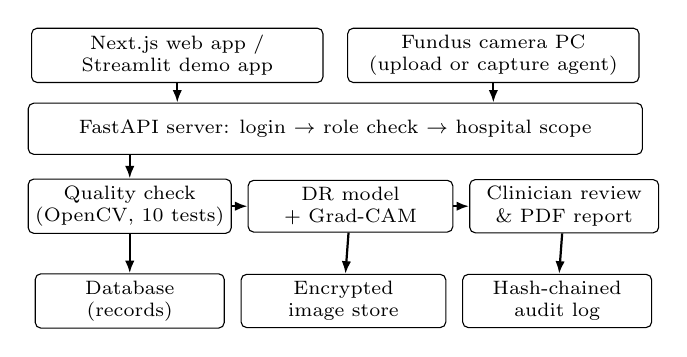
\begin{tikzpicture}[font=\scriptsize, node distance=3.5mm and 3mm,
  box/.style={draw, rounded corners=2pt, align=center, minimum height=6.5mm, inner sep=2.5pt, fill=white},
  arr/.style={-{Latex[length=1.6mm]}, thick}]
\node[box, minimum width=37mm] (web) {Next.js web app /\\ Streamlit demo app};
\node[box, right=of web, minimum width=37mm] (cam) {Fundus camera PC\\ (upload or capture agent)};
\node[box, below=6mm of $(web)!0.5!(cam)$, minimum width=78mm] (api) {FastAPI server: login $\rightarrow$ role check $\rightarrow$ hospital scope};
\node[box, below=3mm of api.south west, anchor=north west, minimum width=24mm] (iqa) {Quality check\\ (OpenCV, 10 tests)};
\node[box, right=2mm of iqa, minimum width=26mm] (ai) {DR model\\ + Grad-CAM};
\node[box, right=2mm of ai, minimum width=24mm] (rep) {Clinician review\\ \& PDF report};
\node[box, below=5mm of iqa, minimum width=24mm] (db) {Database\\ (records)};
\node[box, right=2mm of db, minimum width=26mm] (obj) {Encrypted\\ image store};
\node[box, right=2mm of obj, minimum width=24mm] (aud) {Hash-chained\\ audit log};
\draw[arr] (web) -- (web|-api.north);
\draw[arr] (cam) -- (cam|-api.north);
\draw[arr] (api.south-|iqa) -- (iqa);
\draw[arr] (iqa) -- (ai);
\draw[arr] (ai) -- (rep);
\draw[arr] (iqa) -- (db);
\draw[arr] (ai) -- (obj);
\draw[arr] (rep) -- (aud);
\end{tikzpicture}
\caption{Components of NetraRakshak.}
\label{fig:arch}
\end{figure}

A screening proceeds as follows. Reception registers the patient and records consent for screening and, separately, for
AI analysis. The technician uploads the right- and left-eye images. Ten quality tests run on each image
(Table~\ref{tab:iqa}); a failed test returns ``recapture required'' and the reason. The model runs only on images that
pass, and only if AI consent is on record. The ophthalmologist then sees the images, the model's probabilities and the
Grad-CAM map, records a grade per eye, and signs by re-entering their password. A report generated before signing is
watermarked ``draft''; after signing it is marked ``clinician approved'' and the screening is locked. The model's
output is stored in its own table and is never overwritten by the doctor's grade.

Each hospital's records are kept separate in every database query, staff have one of five roles, images and reports
are encrypted before storage, and every view, upload, analysis and signature is written to an audit log in which each
entry includes a SHA-256 hash of the previous one.

\begin{table}[t]
\caption{Image Quality Tests (run before the model)}
\label{tab:iqa}
\centering\scriptsize
\begin{tabular}{@{}ll@{}}
\toprule
Test & What is measured \\
\midrule
Resolution & shorter side $\geq$ 512 pixels \\
Retinal visibility & share of the frame covered by the retina \\
Field of view & distance of the retina's centre from the image centre \\
Fundus plausibility & red channel dominant inside the retina \\
Brightness & mean luminance inside the retina \\
Contrast & standard deviation of the green channel \\
Exposure & share of over- and under-exposed pixels \\
Blur & variance of the Laplacian \\
Focus & mean squared Sobel gradient \\
Artefacts & uneven illumination, large reflections \\
\bottomrule
\end{tabular}
\end{table}

\section{Model Development}
\subsection{Data and Split}
APTOS 2019~\cite{aptos2019} contains 3,662 colour fundus images from Aravind Eye Hospital, each graded 0--4 on the
International Clinical DR scale~\cite{wilkinson2003}. We used it under the Kaggle competition rules accepted by our
account; we have not confirmed that it may be used in a commercial product. We split the images approximately 71/14/14 into training,
validation and test sets with scikit-learn's \texttt{StratifiedGroupKFold} (random seed 42), stratified by grade
(Table~\ref{tab:data}). The splitting code groups images by patient, but APTOS does not publish patient identifiers, so
each image formed its own group. We return to this in Section~\ref{sec:threats}.

\begin{table}[t]
\caption{Images per Grade in Each Split}
\label{tab:data}
\centering\scriptsize
\begin{tabular}{@{}lrrrrrr@{}}
\toprule
Split & No DR & Mild & Moderate & Severe & PDR & Total \\
\midrule
Train & 1281 & 281 & 710 & 134 & 209 & 2615 \\
Validation & 251 & 43 & 156 & 34 & 39 & 523 \\
Test & 273 & 46 & 133 & 25 & 47 & 524 \\
\bottomrule
\end{tabular}
\end{table}

\subsection{Preprocessing}
Each image is cropped to the circular retina, padded to a square and resized to $384\times384$. We then subtract a
Gaussian-blurred copy, $I' = 4I - 4\,(G_\sigma * I) + 128$ with $\sigma = 384/30$, as Graham did in the 2015 Kaggle
competition~\cite{graham2015}; this evens out illumination differences between cameras. Pixels are scaled with the
ImageNet mean and standard deviation. Inference uses the same function as training. During training, images are
randomly flipped, rotated (up to $\pm180^\circ$), rescaled (0.92--1.10) and given small brightness and contrast changes.

\subsection{Network and Training}
We used EfficientNet-B0~\cite{tan2019} from torchvision with ImageNet weights~\cite{deng2009}, replacing the classifier
with dropout ($p=0.3$) and a linear layer with five outputs (4.01\,M parameters in total). The loss was cross-entropy
with label smoothing 0.05 and class weights inversely proportional to class frequency, to counter the dominance of
grade~0. We trained with AdamW (learning rate $3\times10^{-4}$, weight decay $10^{-4}$), a one-cycle learning-rate
schedule, batch size 24 and mixed precision, for at most 25 epochs, keeping the checkpoint with the best validation
quadratic weighted kappa~\cite{cohen1968} and stopping after six epochs without improvement.

Training ran in a Kaggle notebook on one NVIDIA GPU with PyTorch 2.11.0 and Python 3.13. It stopped after 14 epochs
and kept epoch 8 (validation kappa 0.887). The first epoch took 244\,s because it also preprocessed and cached the
images; later epochs took about 24\,s, for 9.3 minutes in total. Fig.~\ref{fig:curve} shows the logged training loss
and validation kappa. The validation kappa peaks early and then fluctuates while the training loss keeps falling, a
sign that longer training would mainly have fitted the training set more closely.

\begin{figure}[t]
\centering
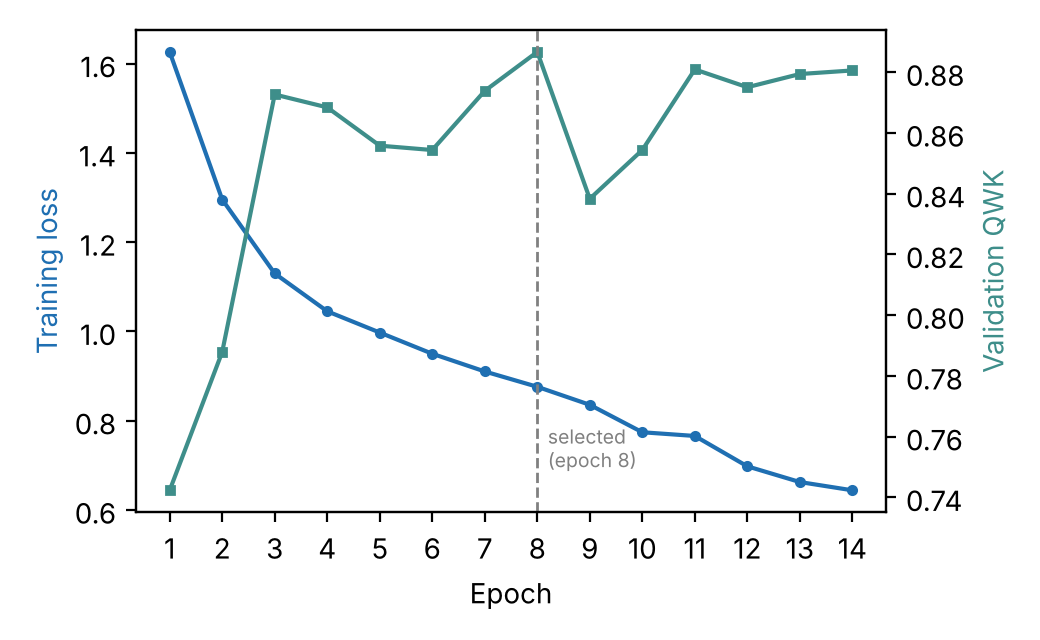
\includegraphics[width=0.95\columnwidth]{figures/training_curve.png}
\caption{Training loss and validation quadratic weighted kappa per epoch (values logged by the training script).}
\label{fig:curve}
\end{figure}

\subsection{Calibration and Withholding Uncertain Grades}
Softmax outputs of modern networks tend to be over-confident~\cite{guo2017}. We fitted a single temperature $T$ to the
validation logits by minimising the negative log-likelihood (L-BFGS), obtaining $T=0.771$. In use, the probabilities
are $p_k = \mathrm{softmax}(z/T)_k$. The application shows the top grade only if its probability is at least 0.60 and
the normalised entropy $-\sum_k p_k\log p_k/\log 5$ is at most 0.75; otherwise it shows ``inconclusive --- human review
required''. These thresholds are defaults and have not yet been tuned on the validation set.

\subsection{Grad-CAM Implementation}
For each analysed image we compute Grad-CAM~\cite{selvaraju2017} on the output of the last convolutional block of
EfficientNet-B0 (\texttt{features[-1]}, a $12\times12$ feature map with 1,280 channels at our input size). A forward
hook stores the activations $A^k$ and a backward hook stores the gradients of the predicted class's logit $y^c$. The
weight of each channel is the spatial mean of its gradient, $\alpha_k = \frac{1}{144}\sum_{i,j}\partial y^c/\partial
A^k_{ij}$, and the map is $\mathrm{ReLU}(\sum_k \alpha_k A^k)$, divided by its maximum. The map is enlarged to
$512\times512$ with bicubic interpolation, coloured with the JET colour map and blended with the photograph (42\% map,
58\% image). Both the overlay and the plain heatmap are stored, encrypted, alongside the result. The interface and the
PDF label them as an explanation of the model's output, not as detected lesions.

\section{Results}
\subsection{Test-Set Performance}
All values below come from the 524 test images, which were not used for training, for choosing the checkpoint or for
fitting the temperature. The training script computed them from the saved predictions and wrote them into the model's
metadata file. Fig.~\ref{fig:cm} shows the confusion matrix. Its diagonal holds $271+33+86+11+28 = 429$ correct
grades, so the accuracy is $429/524 = 81.9\%$. For the referable/non-referable decision, grades 2--4 are pooled: 168 of
the 205 referable test images were predicted as grade 2 or higher (sensitivity 82.0\%), and 308 of the 319
non-referable images as grade 0 or 1 (specificity 96.6\%). Confidence intervals in Table~\ref{tab:metrics} are 95\%
Wilson intervals. They come from a single training run; we did not repeat training with other seeds.

\begin{table}[t]
\caption{Test-Set Results (n = 524, one training run)}
\label{tab:metrics}
\centering\scriptsize
\begin{tabular}{@{}lr@{}}
\toprule
Measure & Value (95\% CI) \\
\midrule
Accuracy, 5 grades & 81.9\% (78.3--84.9) \\
Quadratic weighted kappa & 0.876 \\
Macro F1 & 0.670 \\
Macro ROC-AUC (one-vs-rest) & 0.917 \\
\midrule
Referable DR sensitivity & 82.0\% (76.1--86.6), 168/205 \\
Referable DR specificity & 96.6\% (93.9--98.1), 308/319 \\
Referable DR PPV / NPV & 93.9\% / 89.3\% \\
Referable DR ROC-AUC & 0.981 \\
\midrule
Calibration error (ECE), before / after & 12.2\% / 6.1\% \\
\bottomrule
\end{tabular}
\end{table}

\begin{table}[t]
\caption{Results per Grade}
\label{tab:perclass}
\centering\scriptsize
\begin{tabular}{@{}lrrrrr@{}}
\toprule
Grade (test images) & Sens. & Spec. & Prec. & F1 & AUC \\
\midrule
No DR (273) & 99.3\% & 96.8\% & 97.1\% & 0.982 & 0.998 \\
Mild NPDR (46) & 71.7\% & 93.1\% & 50.0\% & 0.589 & 0.935 \\
Moderate NPDR (133) & 64.7\% & 93.1\% & 76.1\% & 0.699 & 0.946 \\
Severe NPDR (25) & 44.0\% & 95.8\% & 34.4\% & 0.386 & 0.810 \\
Proliferative DR (47) & 59.6\% & 98.7\% & 82.4\% & 0.691 & 0.895 \\
\bottomrule
\end{tabular}
\end{table}

\begin{figure*}[t]
\centering
\includegraphics[height=6.2cm]{figures/confusion_matrix.png}\hspace{1.2cm}
\includegraphics[height=6.2cm]{figures/roc_curves.png}
\caption{Test set (n = 524): confusion matrix (left; rows are reference grades) and ROC curves (right).}
\label{fig:cm}
\end{figure*}

The model is reliable at recognising eyes without retinopathy (271 of 273). Most of its errors are between neighbouring
grades: 26 moderate cases were called mild, and 12 severe cases were called moderate. Severe NPDR, with only 25 test
images, is the weakest grade (11 correct; sensitivity CI 26.7--62.9\%).

\subsection{Speed}
On a two-core 2.1\,GHz Intel Xeon CPU with no GPU, one analysis including Grad-CAM took a median of 304\,ms
(90th percentile 331\,ms over 10 runs), and the ten quality tests took about 73\,ms.

\subsection{Does the Workflow Work?}
We tested the software at three levels. First, 30 automated tests check, among other things: that one hospital cannot
read another's records; that each role is refused actions outside its permissions; that blurred, dark, low-resolution
and non-fundus images are rejected; that no AI result is produced without consent, for a failed image, when no model is
installed, or when the model file's SHA-256 does not match its metadata; that an uncertain prediction is shown as
inconclusive; that signing fails without the attestation or with a wrong password; that a report is ``draft'' before
signing and ``clinician approved'' after; and that the audit hash chain verifies. All 30 pass. Second, a scripted
browser session completed the whole workflow (registration, upload of both eyes, quality check, analysis with this
model, review, signature, PDF, dashboard) against the server running in production mode on PostgreSQL. Third, the same
sequence was repeated through the Streamlit demo. Fig.~\ref{fig:ui} shows the review screen from the first front end.

\begin{figure}[t]
\centering
\includegraphics[width=\columnwidth]{figures/ui_review.png}
\caption{Clinician review screen with a synthetic test patient: Grad-CAM overlay, the model's probabilities, and the
per-eye accept/modify/reject controls.}
\label{fig:ui}
\end{figure}

\section{Threats to Validity}
\label{sec:threats}
\textit{Leakage between splits.} Because APTOS lacks patient identifiers, the two eyes of one person, or repeated
photographs of the same eye, may sit in different splits. Near-duplicate images in APTOS have also been reported by
Kaggle participants; we did not check for them. Both effects would make the test results look better than they are. A per-patient split on a dataset
with identifiers, plus duplicate detection by perceptual hashing, is needed before the numbers can be trusted.

\textit{Single source.} All images come from one hospital network. Performance on other cameras, populations, or
undilated pupils is unknown; we have not evaluated on an external set such as IDRiD~\cite{porwal2018}.

\textit{Single run.} The intervals in Table~\ref{tab:metrics} describe sampling of the test set only, not variation
between training runs.

\textit{Inputs outside the training distribution.} The quality tests check image properties, not whether the image is a
retina the model has learned to grade. When we fed the model procedurally generated synthetic test images, it returned
confident grades. An out-of-distribution check is needed.

\textit{Missed referable cases.} At the default operating point, 37 of 205 referable eyes (18\%) were graded
non-referable. This is the main reason the software requires a clinician's signature on every case.

\section{Reproducibility}
The model file used for all results has SHA-256
\texttt{d25443af\ldots eaad9b}; the application refuses to load it if the hash differs. Its metadata file stores the
split sizes, per-epoch history, temperature and every metric reported here. The split is deterministic given the
APTOS label file and seed 42. Retraining takes one command (\texttt{python -m ai.modules.diabetic\_retinopathy.train}
with the arguments above, or the provided Kaggle notebook script), and \texttt{evaluate.py} re-scores a saved model on
any labelled set. The source code, model metadata and test suite are available from the authors on request.

\section{Regulatory and Ethical Notes}
In India, software intended to screen for disease is a medical device under the Medical Devices Rules, 2017. CDSCO's
draft guidance on medical device software (October 2025) asks for lifecycle quality management, risk management,
clinical evaluation and a protocol for changing AI models after approval~\cite{cdsco2025}. We prepared draft
intended-use, risk (ISO~14971~\cite{iso14971}) and software documents with IEC~62304~\cite{iec62304} in mind, and
consent and erasure follow the Digital Personal Data Protection Act, 2023~\cite{dpdp2023}. None of this has been
assessed by a regulator. All patients and images shown in this paper are synthetic.

\section{Conclusion}
An EfficientNet-B0 model trained for under ten minutes on APTOS 2019 reached 81.9\% five-grade accuracy and 82.0\% /
96.6\% sensitivity/specificity for referable DR on a held-out split, and we placed it inside a workflow where it can only
suggest. The most important next steps are a per-patient split with duplicates removed, evaluation on images from
other hospitals and cameras, tuning the ``inconclusive'' threshold, and an out-of-distribution check, followed by a
prospective study with ethics approval.

\section*{Acknowledgment}
APTOS 2019 data were provided by the Asia Pacific Tele-Ophthalmology Society through Kaggle. Parts of the software
and of this manuscript were drafted with the help of an AI assistant (Claude, Anthropic); the authors ran the training
and evaluation, checked the results and are responsible for the content.

\begin{thebibliography}{99}
\bibitem{gulshan2016} V.~Gulshan \textit{et al.}, ``Development and validation of a deep learning algorithm for
detection of diabetic retinopathy in retinal fundus photographs,'' \textit{JAMA}, vol.~316, no.~22, pp.~2402--2410, 2016.
\bibitem{ting2017} D.~S.~W.~Ting \textit{et al.}, ``Development and validation of a deep learning system for diabetic
retinopathy and related eye diseases using retinal images from multiethnic populations with diabetes,''
\textit{JAMA}, vol.~318, no.~22, pp.~2211--2223, 2017.
\bibitem{abramoff2018} M.~D.~Abr\`amoff, P.~T.~Lavin, M.~Birch, N.~Shah, and J.~C.~Folk, ``Pivotal trial of an
autonomous AI-based diagnostic system for detection of diabetic retinopathy in primary care offices,''
\textit{npj Digit. Med.}, vol.~1, art.~39, 2018.
\bibitem{ruamviboonsuk2019} P.~Ruamviboonsuk \textit{et al.}, ``Deep learning versus human graders for classifying
diabetic retinopathy severity in a nationwide screening program,'' \textit{npj Digit. Med.}, vol.~2, art.~25, 2019.
\bibitem{rajalakshmi2018} R.~Rajalakshmi \textit{et al.}, ``Automated diabetic retinopathy detection in smartphone-based
fundus photography using artificial intelligence,'' \textit{Eye}, vol.~32, pp.~1138--1144, 2018.
\bibitem{aptos2019} Asia Pacific Tele-Ophthalmology Society, ``APTOS 2019 Blindness Detection,'' Kaggle, 2019.
[Online]. Available: \url{https://www.kaggle.com/competitions/aptos2019-blindness-detection}
\bibitem{porwal2018} P.~Porwal \textit{et al.}, ``Indian Diabetic Retinopathy Image Dataset (IDRiD): A database for
diabetic retinopathy screening research,'' \textit{Data}, vol.~3, no.~3, art.~25, 2018.
\bibitem{wilkinson2003} C.~P.~Wilkinson \textit{et al.}, ``Proposed international clinical diabetic retinopathy and
diabetic macular edema disease severity scales,'' \textit{Ophthalmology}, vol.~110, no.~9, pp.~1677--1682, 2003.
\bibitem{graham2015} B.~Graham, ``Kaggle diabetic retinopathy detection competition report,'' Univ. of Warwick, 2015.
\bibitem{tan2019} M.~Tan and Q.~V.~Le, ``EfficientNet: Rethinking model scaling for convolutional neural networks,''
in \textit{Proc. 36th Int. Conf. Mach. Learn. (ICML)}, 2019, pp.~6105--6114.
\bibitem{deng2009} J.~Deng, W.~Dong, R.~Socher, L.-J.~Li, K.~Li, and L.~Fei-Fei, ``ImageNet: A large-scale
hierarchical image database,'' in \textit{Proc. IEEE Conf. Comput. Vis. Pattern Recognit. (CVPR)}, 2009, pp.~248--255.
\bibitem{cohen1968} J.~Cohen, ``Weighted kappa: Nominal scale agreement with provision for scaled disagreement or
partial credit,'' \textit{Psychol. Bull.}, vol.~70, no.~4, pp.~213--220, 1968.
\bibitem{guo2017} C.~Guo, G.~Pleiss, Y.~Sun, and K.~Q.~Weinberger, ``On calibration of modern neural networks,'' in
\textit{Proc. 34th Int. Conf. Mach. Learn. (ICML)}, 2017, pp.~1321--1330.
\bibitem{selvaraju2017} R.~R.~Selvaraju, M.~Cogswell, A.~Das, R.~Vedantam, D.~Parikh, and D.~Batra, ``Grad-CAM: Visual
explanations from deep networks via gradient-based localization,'' in \textit{Proc. IEEE Int. Conf. Comput. Vis.
(ICCV)}, 2017, pp.~618--626.
\bibitem{cdsco2025} Central Drugs Standard Control Organisation, ``Draft guidance document on medical device
software,'' Ministry of Health and Family Welfare, Govt. of India, Oct. 2025.
\bibitem{iso14971} \textit{Medical Devices --- Application of Risk Management to Medical Devices}, ISO 14971:2019.
\bibitem{iec62304} \textit{Medical Device Software --- Software Life Cycle Processes}, IEC 62304:2006+A1:2015.
\bibitem{dpdp2023} \textit{The Digital Personal Data Protection Act, 2023}, Act No.~22 of 2023, Govt. of India.
\end{thebibliography}

\end{document}
